\documentclass[border=10pt]{standalone}
\usepackage{pgfplots}
\pgfplotsset{compat=1.18}
\begin{document}
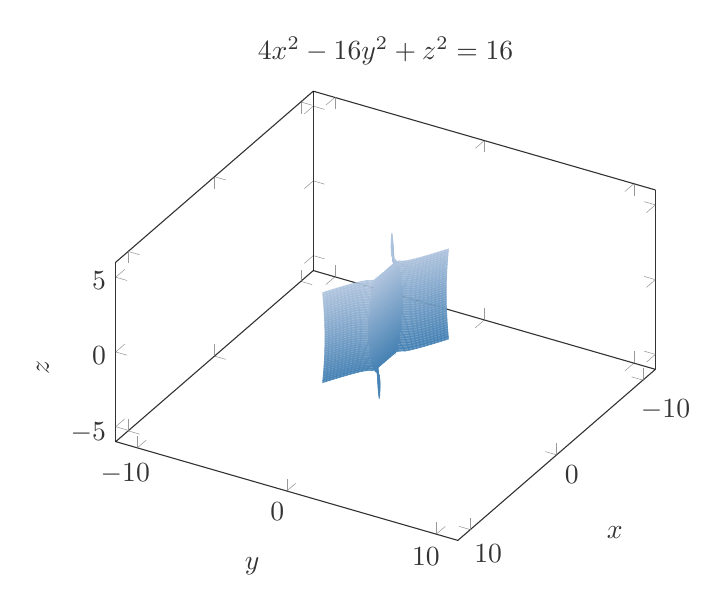
\begin{tikzpicture}
\begin{axis}[
    view={120}{30},
    xlabel=$x$,
    ylabel=$y$,
    zlabel=$z$,
    title={$4x^2-16y^2+z^2=16$},
    xmin=-4, xmax=4,
    ymin=-3, ymax=3,
    zmin=-6, zmax=6,
    samples=40,
    samples y=40,
    colormap={steelblue}{rgb255=(70,130,180) rgb255=(176,196,222)},
    shader=flat,
    opacity=0.8,
    axis equal
]
\addplot3[surf,domain=-4:4,y domain=-3:3,variable=\u,variable y=\v]
    ({u}, {sqrt(max((4*u^2+v^2-16)/16,0))}, {v});
\addplot3[surf,domain=-4:4,y domain=-3:3,variable=\u,variable y=\v]
    ({u}, {-sqrt(max((4*u^2+v^2-16)/16,0))}, {v});
\end{axis}
\end{tikzpicture}
\end{document}
